
\documentclass[12pt]{article}

\usepackage{xeCJK}%字體設定
\setCJKmainfont{cwTeXKai}
% \setCJKmainfont{cwTeXKai}[AutoFakeBold=1.5]


\setmainfont{Times New Roman}  % 英文正文字體

\usepackage[top=2cm,bottom=2cm,left=2cm,right=2cm,a4paper]{geometry}%版面設定

\usepackage{indentfirst}%縮排

\usepackage{setspace}%行距設計
\onehalfspacing%半行距
\setlength{\parskip}{3pt}%段落之間

\usepackage{moresize}%字體大小

\usepackage{graphicx}

\usepackage{amssymb}%數學符號

\usepackage{amsmath} % 數學符號
\usepackage{booktabs}         % 漂亮的表格（\toprule, \midrule, \bottomrule）
\usepackage{siunitx}          % 國際單位制 (建議處理單位更漂亮)

\usepackage{multicol}%引入函數使下面那些可以變成雙欄

\usepackage{float}%圖片固定

% \renewcommand{\thesection}{\Roman{section}}


%%%%%%%%%%%%%%%%%%%%%%%%%%%%%%正文%%%%%%%%%%%%%%%%%%%%%%%%%%%%%%%%%%%
\begin{document}

\begin{titlepage}
\begin{center}

\vspace*{0.5cm}
\HUGE \textbf{General Physics Lab Report}\\
\vspace{1cm}
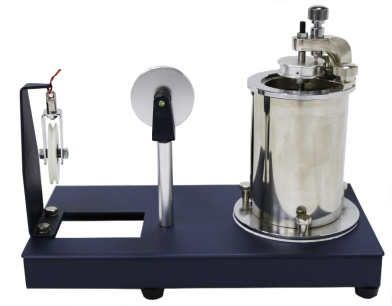
\includegraphics[width=9cm]{IMG_0367.jpeg}\\[0.5cm]
\HUGE \textbf{Viscosity Coefficient}\\

\vfill
\huge Group 3 \\[0.25cm]
\begin{table}[h]
\centering
\Large
\begin{tabular}{|c|c|}
\hline
組員:              & 貢獻度  \\
吳育伭(4114064131) & 33\% \\
卓峻陞(4114064123) & 33\% \\
程鈞寶(4114064132) & 33\% \\ \hline
\end{tabular}
\end{table}

\end{center}

\end{titlepage}

%%%%%%%%%%%%%%%%%%%%%%%%%%%%%%%%%%%%%%%%%%%%%%%%%%%%%%%%%%%%%%%%
\section*{\textbf{Questions of Discussion}}
\large
\noindent
$Q1:$ 
\textbf{What are the sources of error in this experiment?}\\
$A:$
The friction between the threads and the pulley may have reduced the speed. And sometimes, cause it to get stuck too.
For experiment 2, the heat loss from the container is too fast, causing the temperature to drop quite quickly when we are experimenting. The cooling speed may be influenced by the AC.
\\
Glycerin is also prone to moisture. Easily absorbing water vapor from the air, which causes changes in its concentration and viscosity.\\

\noindent
$Q2:$ 
\textbf{Based on the result obtained in Step 2 of the experiment, explain its effect on daily life. If someone is living in a cold region, should they use oil with a larger or smaller viscosity coefficient for their car (viscosity is measured at room temperature)?}\\
$A:$
In theory, as the temperature decreases, the viscosity coefficient increases. Therefore, using engine oil with a lower viscosity coefficient (while in room temperature),  ensures that the oil will still flow in low temperature, although it will be thicker.\\ 

\noindent
$Q3:$
\textbf{If an unknown liquid does not wet the cylinder used in this experiment, can we still use this method to measure the viscosity coefficient? Why?}\\
$A:$No, we cannot use the original method in this case. Instead, we could use the capillary tube method, which measures the time required for the liquid to flow through a capillary tube and calculates its viscosity. 

Why can't we use our method? Because it will not stick properly, in turn causing air gaps between them. This violates the no-slip condition — with the assumption that the fluid in contact with the wall has zero relative velocity to it.\\

\noindent
$Q4:$
\textbf{Give one example from daily life that relates to viscosity and briefly explain it.} \\
$A:$
Most topical creams is in a gel like form, that is intentionally viscous.  Why? So It can be applied easily and won't make a mess when you drop it. Imagine taking your topical cream, but if the cream's viscosity is like water, it will be very inconvenient.
% ---------------------------------------------------------------------------------------------------
%%%%%%%%%%%%%%%%%%%%%%%%%%%%%%%%%%%%%%%%%%%%%%%%%%%%%%%%%%%%%%%%%%%
\large
\section{\textbf{Objective}}
To learn the ways to measure a liquid's viscosity constant while simultaneously observing its changes to temperatures.

%%%%%%%%%%%%%%%%%%%%%%%%%%%%%%%%%%%%%%%%%%%%%%%%%%%%%%%%%%%%%%%%

% \section{\textbf{Principle}}


%%%%%%%%%%%%%%%%%%%%%%%%%%%%%%%%%%%%%%%%%%%%%%%%%%%%%%%%%%%%%%%%

\section{\textbf{Theory}}
When the weights fall at a constant speed, the gravitational force acting on them ($Mg$) is balanced by the liquid's friction, causing it to pull on the string. And because the velocity is constant, we can deduce that
\[
\Sigma Fy = fdrag-Mg=0
\]
\[
fdrag=Mg
\]

At this point, the torque can be expressed as
\[
\tau = \frac{\eta v}{A}
\]

Since the torque $\tau$ equals to $fdrag$ divided by the cylinder contact area (2πal), we have
\[
\tau = \frac{fdrag }{2 \pi a l}= Mg
\]

Therefore,
\[
\frac{fdrag}{A} = \frac{\eta v}{(b-a)} 
\Rightarrow 
Mg = \frac{\eta v}{(b - a)} (2\pi a l)
\]
\[
M =\frac{\eta v 2\pi a l}{(b-a)g} v
\]
Hence, it can be concluded that
\[
m \propto v
\]
which means the mass of the weights is directly proportional to the terminal velocity.

\begin{align*}
\tau &: \text{Shear stress (\si{\pascal})} \\
\eta &: \text{Viscosity coefficient (\si{\pascal\second})} \\
v &: \text{Velocity (\si{\meter\per\second})} \\
b &: \text{Outer radius of the cylinder (\si{\meter})} \\
a &: \text{Inner radius of the cylinder (\si{\meter})} \\
l &: \text{Height of the cylinder (\si{\meter})} \\
fdrag &: \text{Friction from the liquid that is caused by the mass(\si{\newton})} \\
A &: \text{Contact area (\si{\meter\squared})} \\
M &: \text{Mass of weights (\si{\kilogram})} \\
g &: \text{Acceleration due to gravity (\si{\meter\per\second\squared})}
\end{align*}

\begin{figure}[H]
    \centering
    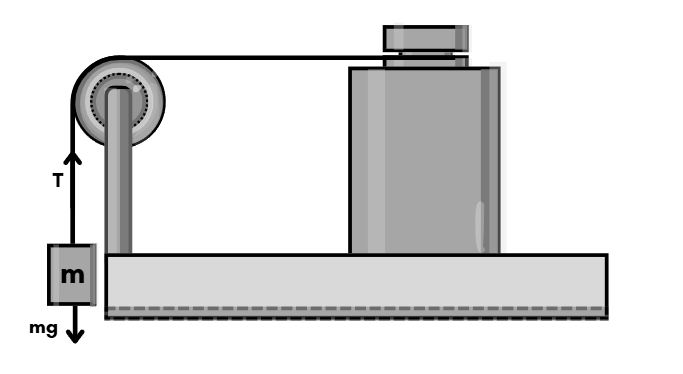
\includegraphics[width=0.5\linewidth]{黏滯係數/黏滯係數/Screenshot 2025-10-07 211215.png}
    \caption{viscosity coefficient test Apparatus}
    \label{fig:理論圖}
\end{figure}
\noindent


%%%%%%%%%%%%%%%%%%%%%%%%%%%%%%%%%%%%%%%%%%%%%%%%%%%%%%%%%%%%%%%%

\section{\textbf{Ways of Experiment}}
The rotational viscometer method is used to measure the viscosity coefficient of glycerin at different temperatures.


% \noindent
% \subsection{\textbf{Experiment 1}：Testing the Viscosity Coefficient in constant Temperature}

% \subsection{\textbf{Experiment 2}：The Viscosity Coefficient of Glycerine in Different Temperature }


%%%%%%%%%%%%%%%%%%%%%%%%%%%%%%%%%%%%%%%%%%%%%%%%%%%%%%%%%%%%%%%%

\section{\textbf{Data Analysis}}

\subsection{The constants in Viscosity Coefficient Apparatus}

\begin{itemize}
    \item Inner radius=$2.800cm$
    \item Outer radius=$2.985cm$
    \item Drum shaft radius=$3.790cm$
    \item The height of the cylinder=$8.180cm$
\end{itemize}

%%%%%%%%%%%%%%%%%%%%%%%%%實驗一%%%%%%%%%%%%%%%%%%%%%%%%%%%%%%%%%%%%
\subsection{\textbf{Experiment 1}：Testing the Viscosity Coefficient in constant Temperature (Arduino)}
Temperature=21$^\circ C$
\begin{table}[H]
\begin{tabular}{|cccc|c|}
\hline
Mass of Weights(g) & Falling Height(cm) & Time(s) & Terminal Velocity(cm/s) & Viscosity Coefficient(cP) \\ \hline
10.27              & 9.96               & 7.13    & 1.40                    & 15.42                 \\
20.30              & 9.96               & 1.70    & 5.87                    & 7.25                  \\
30.19              & 9.96               & 1.25    & 8.44                    & 7.50                  \\
40.2               & 9.96               & 0.80    & 12.51                   & 6.74                  \\
50.3               & 9.96               & 0.64    & 15.75                   & 6.67                  \\ \hline
\end{tabular}
\end{table}
*All time measurements are done by Arduino.
\begin{enumerate}
    \item The average viscosity of glycerin measured (excluding the first data point) is approximately 7.04 cP. This corresponds to a glycerin concentration between 50-60\% .
    \item The ratio of mass to time is around 3.36, which remains nearly constant during our experiments. The viscosity coefficient is approximately 7.04 cP.
\end{enumerate}


\begin{figure}[H]
    \centering
    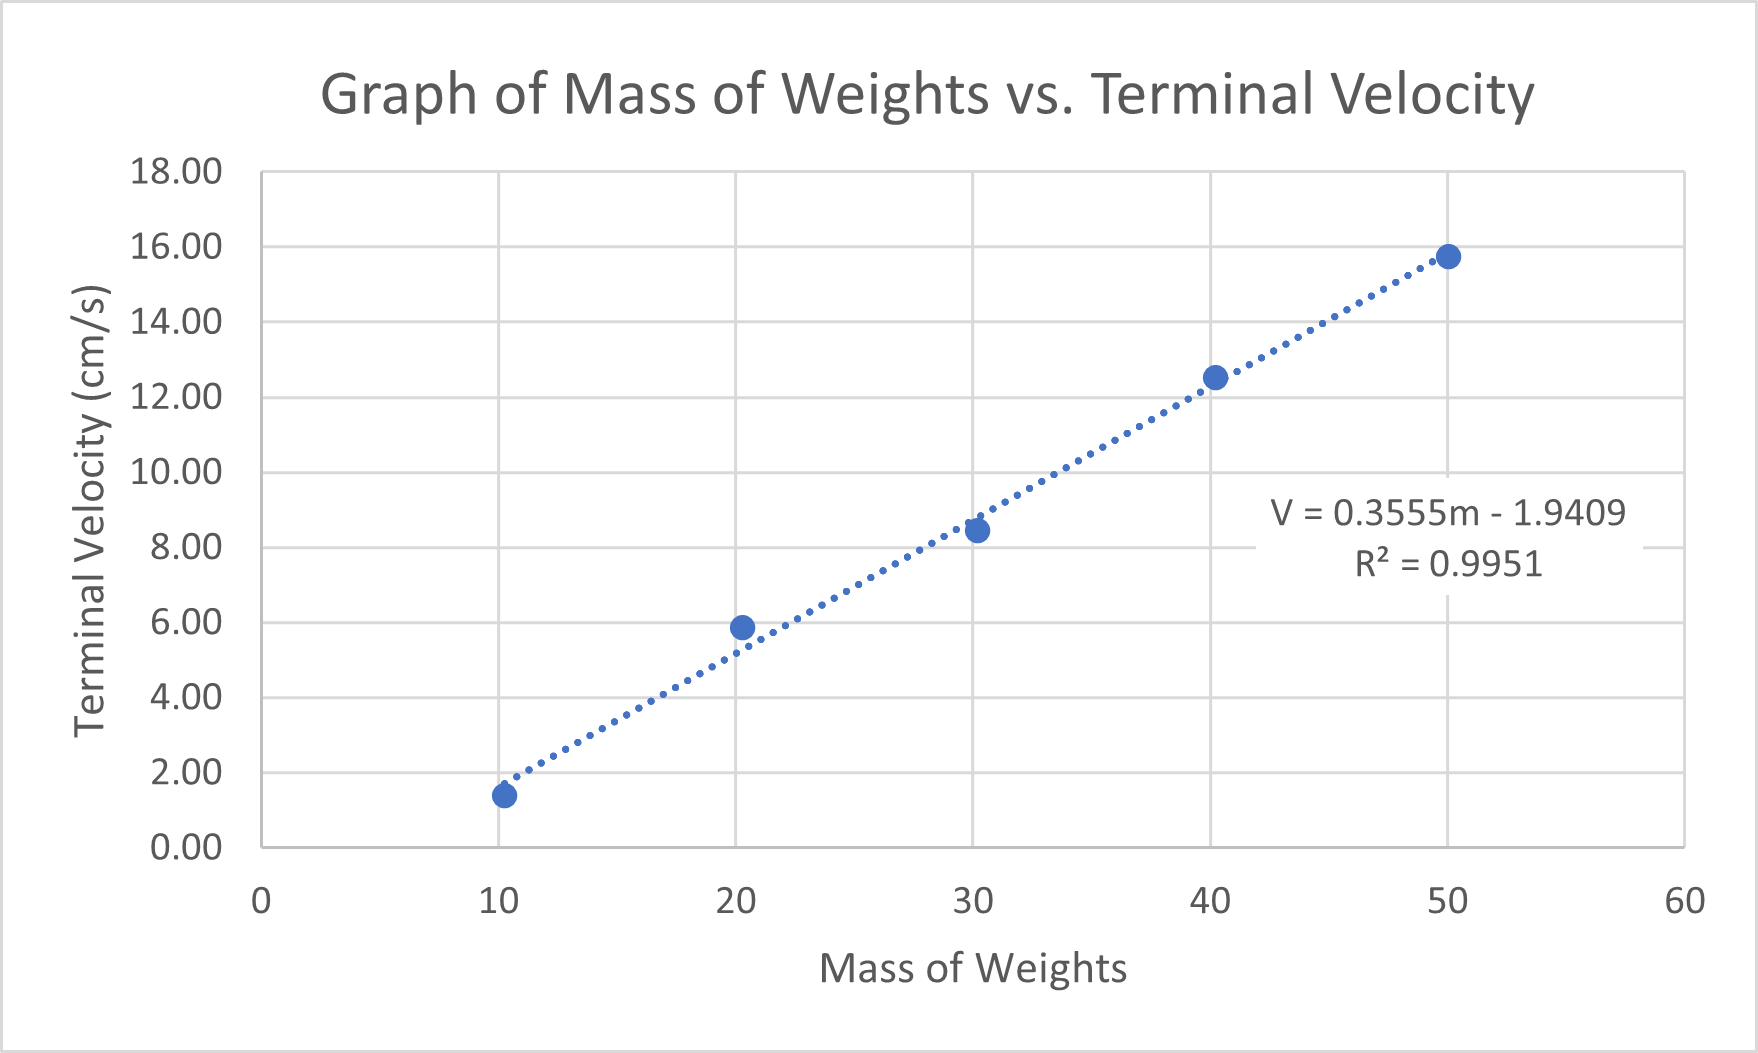
\includegraphics[width=0.7\linewidth]{黏滯係數/實驗一the mass of weights vsterminal velocity.png}
    \caption{The mass of weights vs terminal velocity}
    \label{fig:placeholder}
\end{figure}


%%%%%%%%%%%%%%%%%%%%%%%%%%%%%%實驗二%%%%%%%%%%%%%%%%%%%%%%%%%%%%%%%%%%%%%%%%%%%%%
\subsection{\textbf{Experiment 2}：The Viscosity Coefficient of Glycerin in Different Temperature (Arduino)}

\begin{table}[H]
\begin{tabular}{|cccc|c|}
\hline
Temperature($^\circ C$) & Falling Height(cm) & Time(s) & Terminal Velocity(cm/s) & Viscosity Coefficient \\ \hline
100                     & 9.96               & 0.22    & 45.38                   & 1.85                  \\
90                      & 9.96               & 0.26    & 38.23                   & 2.19                  \\
80                      & 9.96               & 0.20    & 49.06                   & 1.71                  \\
70                      & 9.96               & 0.20    & 49.06                   & 1.71                  \\
60                      & 9.96               & 0.21    & 48.94                   & 1.71                  \\
50                      & 9.96               & 0.25    & 40.24                   & 2.09                  \\ \hline
\end{tabular}
\end{table}
*All time measurements are done by Arduino.
\begin{enumerate}
    \item The viscosity coefficient decreases as the temperature increases. This can be explained by the fact that higher temperatures provide molecules with greater kinetic energy, enabling them to overcome van der Waals forces and hydrogen bonds more easily.

    \item The concentration of glycerin we used was estimated to be between 50-60 \%, but the experimental data showed significant distortion. A more detailed discussion of this issue will be provided in the Result and Discussion.
\end{enumerate}

\begin{figure}[H]
    \centering
    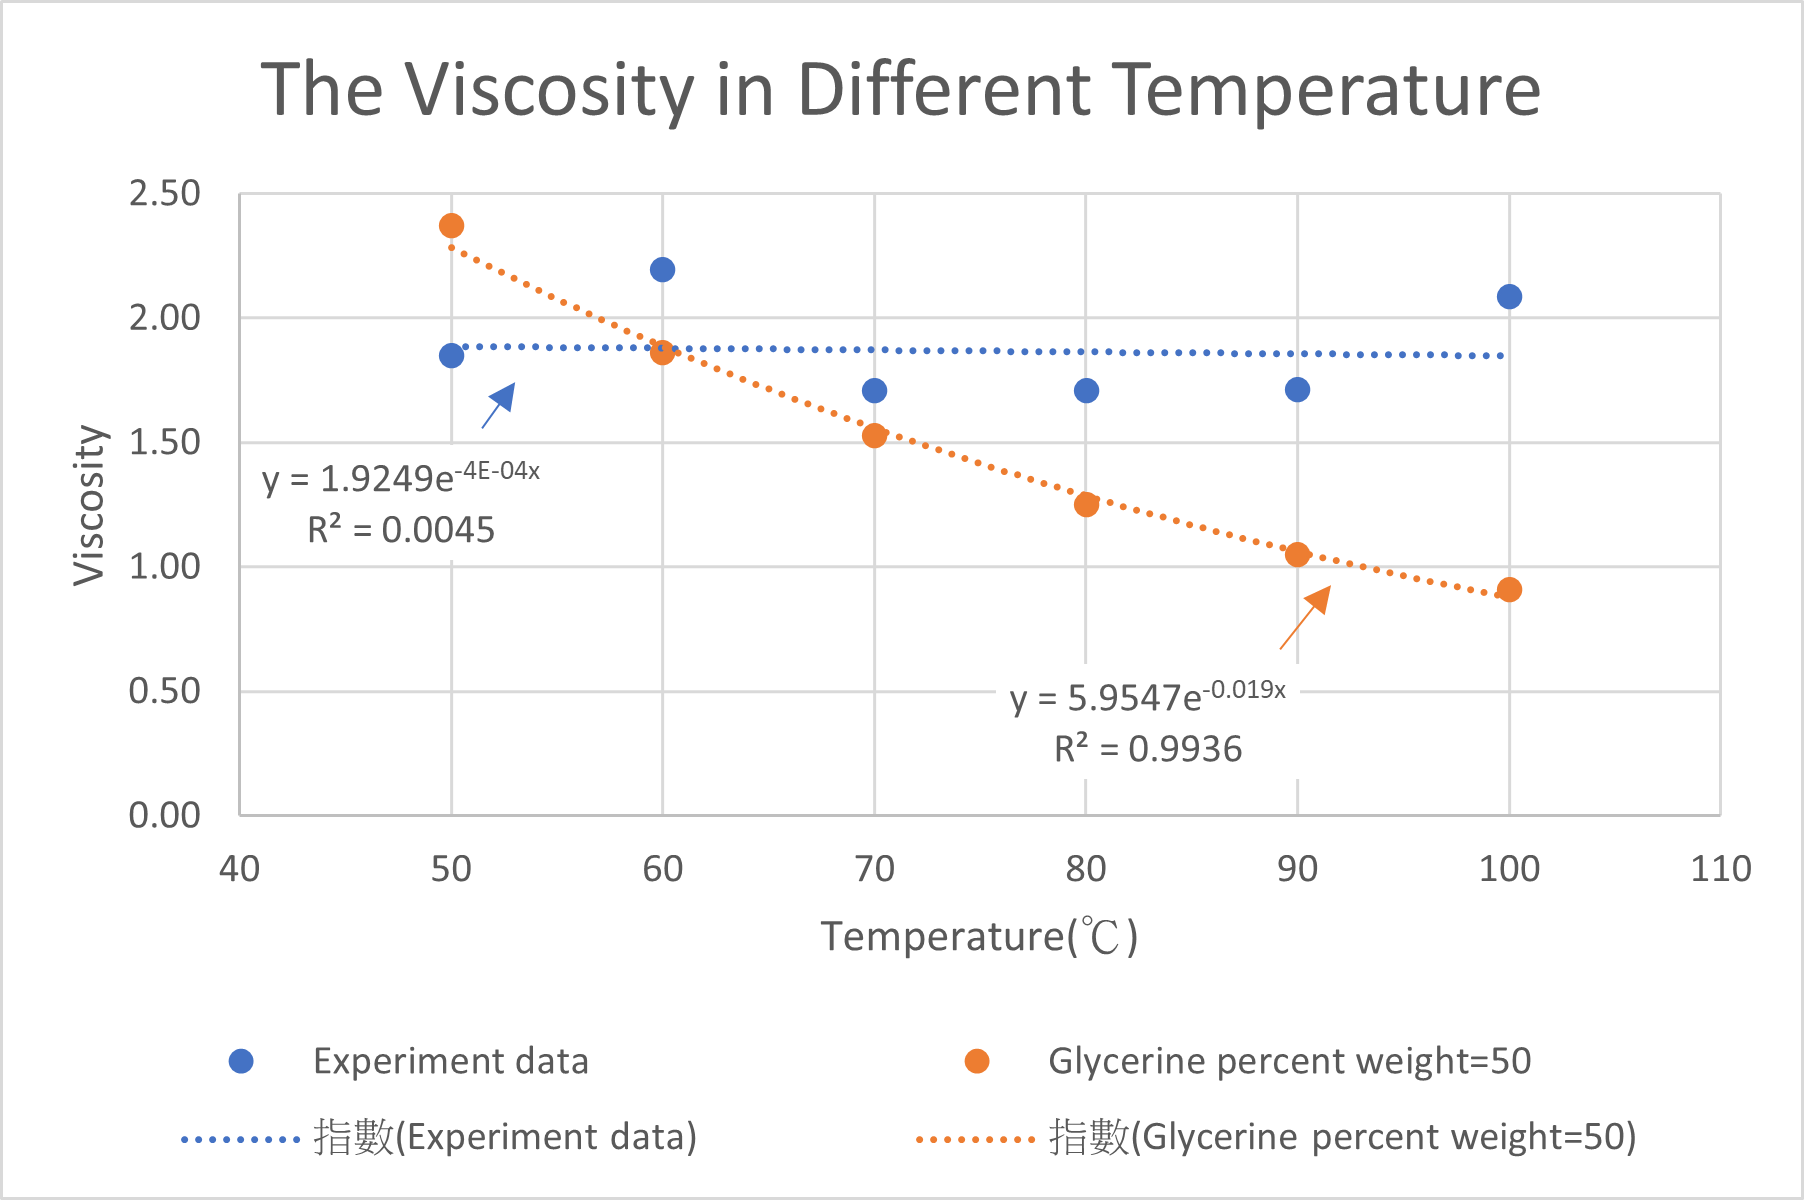
\includegraphics[width=0.7\linewidth]{黏滯係數/實驗二differient temperature.png}
    \caption{Viscosity change in different temperature}
    \label{fig:placeholder}
\end{figure}

%%%%%%%%%%%%%%%%%%%%%%%%%%%%%%%%%%%%%%%%%%%%%%%%%%%%%%%%%%%%%%%%

\section{\textbf{Results and Discussion}}
In this experiment, our second measurement showed that the viscosity values at different temperatures between 50–100 $^\circ C$ (measured every 10 $^\circ C$) were nearly the same. However, theoretically, the viscosity should increase as the temperature decreases.

One possible reason is that, after the process of heating and cooling, the air pressure surrounding the cylinder might  have decreased and some of the surrounding water vapor might have  decided to precipitate. Because glycerin easily absorbs water, its concentration may have been affected by the precipitated water droplets, causing it to change, leading to viscosity values that deviate from the theoretical trend.

Another explanation is that the Arduino-based timer we used can only measure a minimum time interval of about 0.2 s. At higher temperatures, the falling time of the weight approached or even fell below 0.2 s, resulting in significant errors in the calculated viscosity values.

And by far the most likely culprit is—our strings and bearings. The string has always been prone to getting stuck and the bearings have frankly been unreliable. Always getting stuck in the same ways. The friction between the bearings may cause the speed to be the same, and in response, the viscosity constant may become constant as well.

For future experiments, it would be better to conduct measurements in a low-humidity environment and to use a photoelectric timer to reduce the measurement errors. And, as an extra precaution, we will focus on testing the equipment first and pinpointing the possible errors and discrepancies.

% \begin{figure}[H]
%     \centering
%     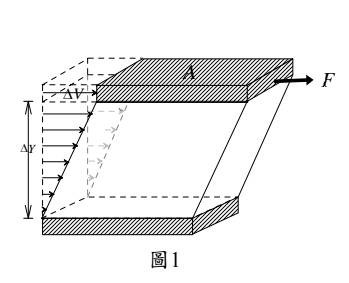
\includegraphics[width=0.5\linewidth]{黏滯係數/黏滯係數/7284.jpg}
%     \caption{Caption}
%     \label{fig:placeholder}
% \end{figure}

% \begin{figure}[H]
%     \centering
%     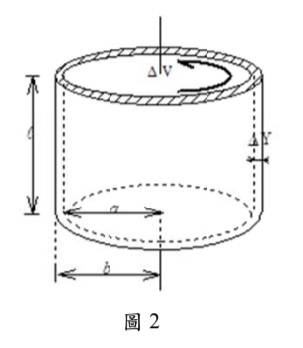
\includegraphics[width=0.5\linewidth]{黏滯係數/黏滯係數/7285.jpg}
%     \caption{Caption}
%     \label{fig:placeholder}
% \end{figure}

%%%%%%%%%%%%%%%%%%%%%%%%%%%%%%%%%%%%%%%%%%%%%%%%%%%%%%%%%%%%%%%%%%%%%%%%%%%%%

\end{document}